% Graphic for TeX using PGF
% Title: /home/emilien/git/g3-bleu-sokoban/rapports/Rapport Phase 2/sequence/Diagramme1.dia
% Creator: Dia v0.97.3
% CreationDate: Sat May  6 12:41:07 2017
% For: emilien
% \usepackage{tikz}
% The following commands are not supported in PSTricks at present
% We define them conditionally, so when they are implemented,
% this pgf file will use them.
\ifx\du\undefined
  \newlength{\du}
\fi
\setlength{\du}{15\unitlength}
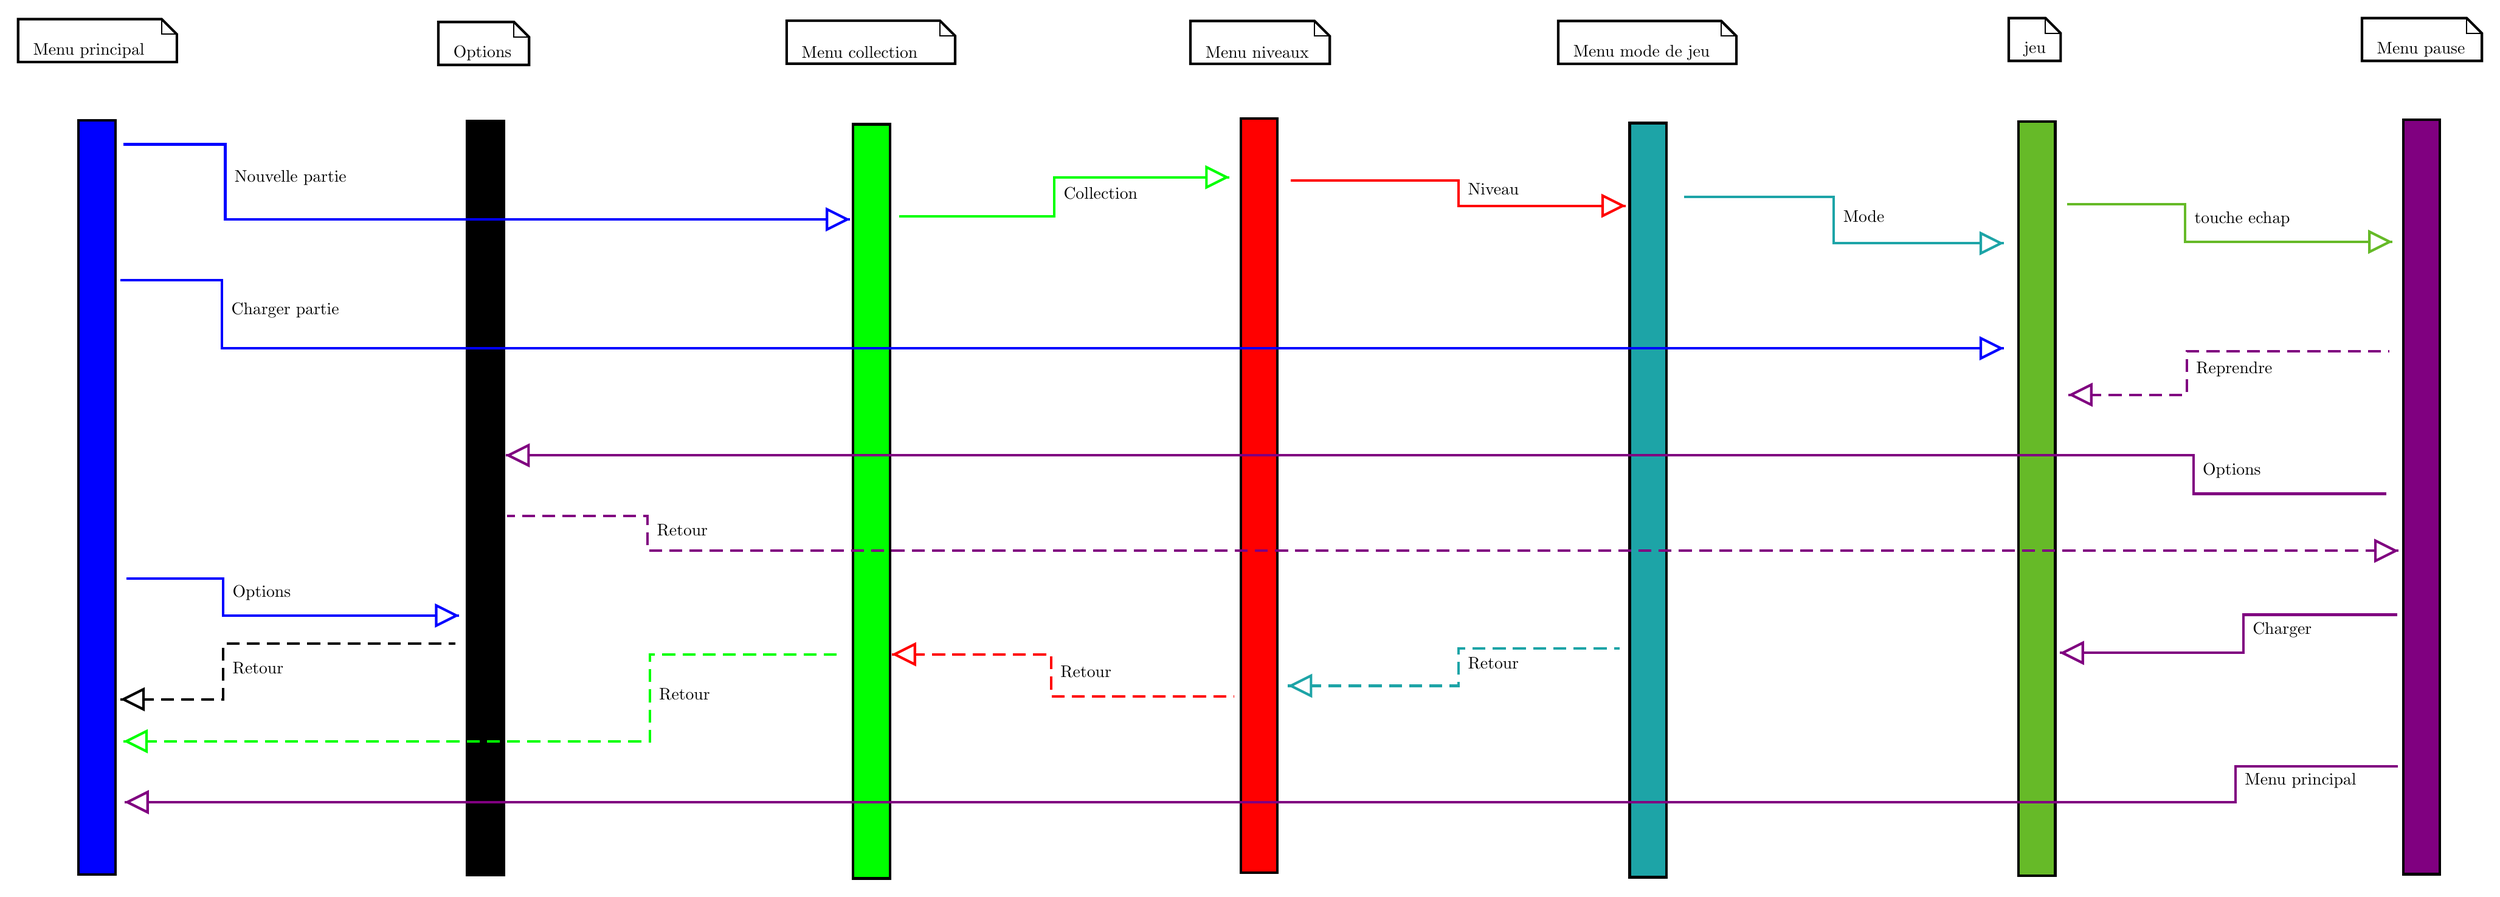
\begin{tikzpicture}
\pgftransformxscale{1.000000}
\pgftransformyscale{-1.000000}
\definecolor{dialinecolor}{rgb}{0.000000, 0.000000, 0.000000}
\pgfsetstrokecolor{dialinecolor}
\definecolor{dialinecolor}{rgb}{1.000000, 1.000000, 1.000000}
\pgfsetfillcolor{dialinecolor}
\pgfsetlinewidth{0.100000\du}
\pgfsetdash{}{0pt}
\pgfsetdash{}{0pt}
\pgfsetmiterjoin
\definecolor{dialinecolor}{rgb}{0.000000, 0.000000, 1.000000}
\pgfsetfillcolor{dialinecolor}
\fill (45.347241\du,5.000000\du)--(45.347241\du,34.898105\du)--(46.797241\du,34.898105\du)--(46.797241\du,5.000000\du)--cycle;
\definecolor{dialinecolor}{rgb}{0.000000, 0.000000, 0.000000}
\pgfsetstrokecolor{dialinecolor}
\draw (45.347241\du,5.000000\du)--(45.347241\du,34.898105\du)--(46.797241\du,34.898105\du)--(46.797241\du,5.000000\du)--cycle;
\pgfsetlinewidth{0.100000\du}
\pgfsetdash{}{0pt}
\definecolor{dialinecolor}{rgb}{1.000000, 1.000000, 1.000000}
\pgfsetfillcolor{dialinecolor}
\fill (42.947241\du,0.987500\du)--(48.637241\du,0.987500\du)--(49.237241\du,1.587500\du)--(49.237241\du,2.687500\du)--(42.947241\du,2.687500\du)--cycle;
\definecolor{dialinecolor}{rgb}{0.000000, 0.000000, 0.000000}
\pgfsetstrokecolor{dialinecolor}
\draw (42.947241\du,0.987500\du)--(48.637241\du,0.987500\du)--(49.237241\du,1.587500\du)--(49.237241\du,2.687500\du)--(42.947241\du,2.687500\du)--cycle;
\pgfsetlinewidth{0.050000\du}
\definecolor{dialinecolor}{rgb}{0.000000, 0.000000, 0.000000}
\pgfsetstrokecolor{dialinecolor}
\draw (48.637241\du,0.987500\du)--(48.637241\du,1.587500\du)--(49.237241\du,1.587500\du);
% setfont left to latex
\definecolor{dialinecolor}{rgb}{0.000000, 0.000000, 0.000000}
\pgfsetstrokecolor{dialinecolor}
\node[anchor=west] at (43.297241\du,2.232500\du){Menu principal};
\pgfsetlinewidth{0.100000\du}
\pgfsetdash{}{0pt}
\definecolor{dialinecolor}{rgb}{1.000000, 1.000000, 1.000000}
\pgfsetfillcolor{dialinecolor}
\fill (59.600000\du,1.100000\du)--(62.595000\du,1.100000\du)--(63.195000\du,1.700000\du)--(63.195000\du,2.800000\du)--(59.600000\du,2.800000\du)--cycle;
\definecolor{dialinecolor}{rgb}{0.000000, 0.000000, 0.000000}
\pgfsetstrokecolor{dialinecolor}
\draw (59.600000\du,1.100000\du)--(62.595000\du,1.100000\du)--(63.195000\du,1.700000\du)--(63.195000\du,2.800000\du)--(59.600000\du,2.800000\du)--cycle;
\pgfsetlinewidth{0.050000\du}
\definecolor{dialinecolor}{rgb}{0.000000, 0.000000, 0.000000}
\pgfsetstrokecolor{dialinecolor}
\draw (62.595000\du,1.100000\du)--(62.595000\du,1.700000\du)--(63.195000\du,1.700000\du);
% setfont left to latex
\definecolor{dialinecolor}{rgb}{0.000000, 0.000000, 0.000000}
\pgfsetstrokecolor{dialinecolor}
\node[anchor=west] at (59.950000\du,2.345000\du){Options};
\pgfsetlinewidth{0.100000\du}
\pgfsetdash{}{0pt}
\definecolor{dialinecolor}{rgb}{1.000000, 1.000000, 1.000000}
\pgfsetfillcolor{dialinecolor}
\fill (73.400000\du,1.050000\du)--(79.475000\du,1.050000\du)--(80.075000\du,1.650000\du)--(80.075000\du,2.750000\du)--(73.400000\du,2.750000\du)--cycle;
\definecolor{dialinecolor}{rgb}{0.000000, 0.000000, 0.000000}
\pgfsetstrokecolor{dialinecolor}
\draw (73.400000\du,1.050000\du)--(79.475000\du,1.050000\du)--(80.075000\du,1.650000\du)--(80.075000\du,2.750000\du)--(73.400000\du,2.750000\du)--cycle;
\pgfsetlinewidth{0.050000\du}
\definecolor{dialinecolor}{rgb}{0.000000, 0.000000, 0.000000}
\pgfsetstrokecolor{dialinecolor}
\draw (79.475000\du,1.050000\du)--(79.475000\du,1.650000\du)--(80.075000\du,1.650000\du);
% setfont left to latex
\definecolor{dialinecolor}{rgb}{0.000000, 0.000000, 0.000000}
\pgfsetstrokecolor{dialinecolor}
\node[anchor=west] at (73.750000\du,2.295000\du){Menu collection};
\pgfsetlinewidth{0.100000\du}
\pgfsetdash{}{0pt}
\definecolor{dialinecolor}{rgb}{1.000000, 1.000000, 1.000000}
\pgfsetfillcolor{dialinecolor}
\fill (89.398874\du,1.060512\du)--(94.318874\du,1.060512\du)--(94.918874\du,1.660512\du)--(94.918874\du,2.760512\du)--(89.398874\du,2.760512\du)--cycle;
\definecolor{dialinecolor}{rgb}{0.000000, 0.000000, 0.000000}
\pgfsetstrokecolor{dialinecolor}
\draw (89.398874\du,1.060512\du)--(94.318874\du,1.060512\du)--(94.918874\du,1.660512\du)--(94.918874\du,2.760512\du)--(89.398874\du,2.760512\du)--cycle;
\pgfsetlinewidth{0.050000\du}
\definecolor{dialinecolor}{rgb}{0.000000, 0.000000, 0.000000}
\pgfsetstrokecolor{dialinecolor}
\draw (94.318874\du,1.060512\du)--(94.318874\du,1.660512\du)--(94.918874\du,1.660512\du);
% setfont left to latex
\definecolor{dialinecolor}{rgb}{0.000000, 0.000000, 0.000000}
\pgfsetstrokecolor{dialinecolor}
\node[anchor=west] at (89.748874\du,2.305512\du){Menu niveaux};
\pgfsetlinewidth{0.100000\du}
\pgfsetdash{}{0pt}
\definecolor{dialinecolor}{rgb}{1.000000, 1.000000, 1.000000}
\pgfsetfillcolor{dialinecolor}
\fill (103.972709\du,1.060512\du)--(110.432709\du,1.060512\du)--(111.032709\du,1.660512\du)--(111.032709\du,2.760512\du)--(103.972709\du,2.760512\du)--cycle;
\definecolor{dialinecolor}{rgb}{0.000000, 0.000000, 0.000000}
\pgfsetstrokecolor{dialinecolor}
\draw (103.972709\du,1.060512\du)--(110.432709\du,1.060512\du)--(111.032709\du,1.660512\du)--(111.032709\du,2.760512\du)--(103.972709\du,2.760512\du)--cycle;
\pgfsetlinewidth{0.050000\du}
\definecolor{dialinecolor}{rgb}{0.000000, 0.000000, 0.000000}
\pgfsetstrokecolor{dialinecolor}
\draw (110.432709\du,1.060512\du)--(110.432709\du,1.660512\du)--(111.032709\du,1.660512\du);
% setfont left to latex
\definecolor{dialinecolor}{rgb}{0.000000, 0.000000, 0.000000}
\pgfsetstrokecolor{dialinecolor}
\node[anchor=west] at (104.322709\du,2.305512\du){Menu mode de jeu};
\pgfsetlinewidth{0.100000\du}
\pgfsetdash{}{0pt}
\definecolor{dialinecolor}{rgb}{1.000000, 1.000000, 1.000000}
\pgfsetfillcolor{dialinecolor}
\fill (121.823730\du,0.944847\du)--(123.278730\du,0.944847\du)--(123.878730\du,1.544847\du)--(123.878730\du,2.644847\du)--(121.823730\du,2.644847\du)--cycle;
\definecolor{dialinecolor}{rgb}{0.000000, 0.000000, 0.000000}
\pgfsetstrokecolor{dialinecolor}
\draw (121.823730\du,0.944847\du)--(123.278730\du,0.944847\du)--(123.878730\du,1.544847\du)--(123.878730\du,2.644847\du)--(121.823730\du,2.644847\du)--cycle;
\pgfsetlinewidth{0.050000\du}
\definecolor{dialinecolor}{rgb}{0.000000, 0.000000, 0.000000}
\pgfsetstrokecolor{dialinecolor}
\draw (123.278730\du,0.944847\du)--(123.278730\du,1.544847\du)--(123.878730\du,1.544847\du);
% setfont left to latex
\definecolor{dialinecolor}{rgb}{0.000000, 0.000000, 0.000000}
\pgfsetstrokecolor{dialinecolor}
\node[anchor=west] at (122.173730\du,2.189847\du){jeu};
\pgfsetlinewidth{0.100000\du}
\pgfsetdash{}{0pt}
\definecolor{dialinecolor}{rgb}{1.000000, 1.000000, 1.000000}
\pgfsetfillcolor{dialinecolor}
\fill (135.819239\du,0.944847\du)--(139.969239\du,0.944847\du)--(140.569239\du,1.544847\du)--(140.569239\du,2.644847\du)--(135.819239\du,2.644847\du)--cycle;
\definecolor{dialinecolor}{rgb}{0.000000, 0.000000, 0.000000}
\pgfsetstrokecolor{dialinecolor}
\draw (135.819239\du,0.944847\du)--(139.969239\du,0.944847\du)--(140.569239\du,1.544847\du)--(140.569239\du,2.644847\du)--(135.819239\du,2.644847\du)--cycle;
\pgfsetlinewidth{0.050000\du}
\definecolor{dialinecolor}{rgb}{0.000000, 0.000000, 0.000000}
\pgfsetstrokecolor{dialinecolor}
\draw (139.969239\du,0.944847\du)--(139.969239\du,1.544847\du)--(140.569239\du,1.544847\du);
% setfont left to latex
\definecolor{dialinecolor}{rgb}{0.000000, 0.000000, 0.000000}
\pgfsetstrokecolor{dialinecolor}
\node[anchor=west] at (136.169239\du,2.189847\du){Menu pause};
\pgfsetlinewidth{0.100000\du}
\pgfsetdash{}{0pt}
\pgfsetdash{}{0pt}
\pgfsetmiterjoin
\definecolor{dialinecolor}{rgb}{0.000000, 0.000000, 0.000000}
\pgfsetfillcolor{dialinecolor}
\fill (60.744159\du,5.027994\du)--(60.744159\du,34.926099\du)--(62.194159\du,34.926099\du)--(62.194159\du,5.027994\du)--cycle;
\definecolor{dialinecolor}{rgb}{0.000000, 0.000000, 0.000000}
\pgfsetstrokecolor{dialinecolor}
\draw (60.744159\du,5.027994\du)--(60.744159\du,34.926099\du)--(62.194159\du,34.926099\du)--(62.194159\du,5.027994\du)--cycle;
\pgfsetlinewidth{0.100000\du}
\pgfsetdash{}{0pt}
\pgfsetdash{}{0pt}
\pgfsetmiterjoin
\definecolor{dialinecolor}{rgb}{0.000000, 1.000000, 0.000000}
\pgfsetfillcolor{dialinecolor}
\fill (76.037189\du,5.152860\du)--(76.037189\du,35.050964\du)--(77.487189\du,35.050964\du)--(77.487189\du,5.152860\du)--cycle;
\definecolor{dialinecolor}{rgb}{0.000000, 0.000000, 0.000000}
\pgfsetstrokecolor{dialinecolor}
\draw (76.037189\du,5.152860\du)--(76.037189\du,35.050964\du)--(77.487189\du,35.050964\du)--(77.487189\du,5.152860\du)--cycle;
\pgfsetlinewidth{0.100000\du}
\pgfsetdash{}{0pt}
\pgfsetdash{}{0pt}
\pgfsetmiterjoin
\definecolor{dialinecolor}{rgb}{1.000000, 0.000000, 0.000000}
\pgfsetfillcolor{dialinecolor}
\fill (91.389678\du,4.920967\du)--(91.389678\du,34.819072\du)--(92.839678\du,34.819072\du)--(92.839678\du,4.920967\du)--cycle;
\definecolor{dialinecolor}{rgb}{0.000000, 0.000000, 0.000000}
\pgfsetstrokecolor{dialinecolor}
\draw (91.389678\du,4.920967\du)--(91.389678\du,34.819072\du)--(92.839678\du,34.819072\du)--(92.839678\du,4.920967\du)--cycle;
\pgfsetlinewidth{0.100000\du}
\pgfsetdash{}{0pt}
\pgfsetdash{}{0pt}
\pgfsetmiterjoin
\definecolor{dialinecolor}{rgb}{0.113725, 0.643137, 0.654902}
\pgfsetfillcolor{dialinecolor}
\fill (106.801626\du,5.105292\du)--(106.801626\du,35.003397\du)--(108.251626\du,35.003397\du)--(108.251626\du,5.105292\du)--cycle;
\definecolor{dialinecolor}{rgb}{0.000000, 0.000000, 0.000000}
\pgfsetstrokecolor{dialinecolor}
\draw (106.801626\du,5.105292\du)--(106.801626\du,35.003397\du)--(108.251626\du,35.003397\du)--(108.251626\du,5.105292\du)--cycle;
\pgfsetlinewidth{0.100000\du}
\pgfsetdash{}{0pt}
\pgfsetdash{}{0pt}
\pgfsetmiterjoin
\definecolor{dialinecolor}{rgb}{0.400000, 0.729412, 0.156863}
\pgfsetfillcolor{dialinecolor}
\fill (122.213575\du,5.051778\du)--(122.213575\du,34.949883\du)--(123.663575\du,34.949883\du)--(123.663575\du,5.051778\du)--cycle;
\definecolor{dialinecolor}{rgb}{0.000000, 0.000000, 0.000000}
\pgfsetstrokecolor{dialinecolor}
\draw (122.213575\du,5.051778\du)--(122.213575\du,34.949883\du)--(123.663575\du,34.949883\du)--(123.663575\du,5.051778\du)--cycle;
\pgfsetlinewidth{0.100000\du}
\pgfsetdash{}{0pt}
\pgfsetdash{}{0pt}
\pgfsetmiterjoin
\definecolor{dialinecolor}{rgb}{0.501961, 0.000000, 0.501961}
\pgfsetfillcolor{dialinecolor}
\fill (137.461397\du,4.982786\du)--(137.461397\du,34.880890\du)--(138.911397\du,34.880890\du)--(138.911397\du,4.982786\du)--cycle;
\definecolor{dialinecolor}{rgb}{0.000000, 0.000000, 0.000000}
\pgfsetstrokecolor{dialinecolor}
\draw (137.461397\du,4.982786\du)--(137.461397\du,34.880890\du)--(138.911397\du,34.880890\du)--(138.911397\du,4.982786\du)--cycle;
\pgfsetlinewidth{0.100000\du}
\pgfsetdash{}{0pt}
\pgfsetmiterjoin
\pgfsetbuttcap
{
\definecolor{dialinecolor}{rgb}{0.000000, 0.000000, 1.000000}
\pgfsetfillcolor{dialinecolor}
% was here!!!
\definecolor{dialinecolor}{rgb}{0.000000, 0.000000, 1.000000}
\pgfsetstrokecolor{dialinecolor}
\draw (75.911023\du,8.925263\du)--(51.156942\du,8.925263\du)--(51.156942\du,5.948100\du)--(47.125411\du,5.948100\du);
}
\definecolor{dialinecolor}{rgb}{0.000000, 0.000000, 1.000000}
\pgfsetstrokecolor{dialinecolor}
\draw (74.999220\du,8.925263\du)--(51.156942\du,8.925263\du)--(51.156942\du,5.948100\du)--(47.125411\du,5.948100\du);
\pgfsetmiterjoin
\definecolor{dialinecolor}{rgb}{1.000000, 1.000000, 1.000000}
\pgfsetfillcolor{dialinecolor}
\fill (74.999220\du,9.325263\du)--(75.799220\du,8.925263\du)--(74.999220\du,8.525263\du)--cycle;
\pgfsetlinewidth{0.100000\du}
\pgfsetdash{}{0pt}
\pgfsetmiterjoin
\definecolor{dialinecolor}{rgb}{0.000000, 0.000000, 1.000000}
\pgfsetstrokecolor{dialinecolor}
\draw (74.999220\du,9.325263\du)--(75.799220\du,8.925263\du)--(74.999220\du,8.525263\du)--cycle;
% setfont left to latex
\definecolor{dialinecolor}{rgb}{0.000000, 0.000000, 0.000000}
\pgfsetstrokecolor{dialinecolor}
\node[anchor=west] at (51.256942\du,7.286681\du){Nouvelle partie};
\pgfsetlinewidth{0.100000\du}
\pgfsetdash{}{0pt}
\pgfsetmiterjoin
\pgfsetbuttcap
{
\definecolor{dialinecolor}{rgb}{0.000000, 0.000000, 1.000000}
\pgfsetfillcolor{dialinecolor}
% was here!!!
\definecolor{dialinecolor}{rgb}{0.000000, 0.000000, 1.000000}
\pgfsetstrokecolor{dialinecolor}
\draw (121.625681\du,14.033775\du)--(51.027632\du,14.033775\du)--(51.027632\du,11.329736\du)--(46.999279\du,11.329736\du);
}
\definecolor{dialinecolor}{rgb}{0.000000, 0.000000, 1.000000}
\pgfsetstrokecolor{dialinecolor}
\draw (120.713878\du,14.033775\du)--(51.027632\du,14.033775\du)--(51.027632\du,11.329736\du)--(46.999279\du,11.329736\du);
\pgfsetmiterjoin
\definecolor{dialinecolor}{rgb}{1.000000, 1.000000, 1.000000}
\pgfsetfillcolor{dialinecolor}
\fill (120.713878\du,14.433775\du)--(121.513878\du,14.033775\du)--(120.713878\du,13.633775\du)--cycle;
\pgfsetlinewidth{0.100000\du}
\pgfsetdash{}{0pt}
\pgfsetmiterjoin
\definecolor{dialinecolor}{rgb}{0.000000, 0.000000, 1.000000}
\pgfsetstrokecolor{dialinecolor}
\draw (120.713878\du,14.433775\du)--(121.513878\du,14.033775\du)--(120.713878\du,13.633775\du)--cycle;
% setfont left to latex
\definecolor{dialinecolor}{rgb}{0.000000, 0.000000, 0.000000}
\pgfsetstrokecolor{dialinecolor}
\node[anchor=west] at (51.127632\du,12.531755\du){Charger partie};
\pgfsetlinewidth{0.100000\du}
\pgfsetdash{}{0pt}
\pgfsetmiterjoin
\pgfsetbuttcap
{
\definecolor{dialinecolor}{rgb}{0.000000, 0.000000, 1.000000}
\pgfsetfillcolor{dialinecolor}
% was here!!!
\definecolor{dialinecolor}{rgb}{0.000000, 0.000000, 1.000000}
\pgfsetstrokecolor{dialinecolor}
\draw (60.426092\du,24.628292\du)--(51.077631\du,24.628292\du)--(51.077631\du,23.156133\du)--(47.231185\du,23.156133\du);
}
\definecolor{dialinecolor}{rgb}{0.000000, 0.000000, 1.000000}
\pgfsetstrokecolor{dialinecolor}
\draw (59.514288\du,24.628292\du)--(51.077631\du,24.628292\du)--(51.077631\du,23.156133\du)--(47.231185\du,23.156133\du);
\pgfsetmiterjoin
\definecolor{dialinecolor}{rgb}{1.000000, 1.000000, 1.000000}
\pgfsetfillcolor{dialinecolor}
\fill (59.514288\du,25.028292\du)--(60.314288\du,24.628292\du)--(59.514288\du,24.228292\du)--cycle;
\pgfsetlinewidth{0.100000\du}
\pgfsetdash{}{0pt}
\pgfsetmiterjoin
\definecolor{dialinecolor}{rgb}{0.000000, 0.000000, 1.000000}
\pgfsetstrokecolor{dialinecolor}
\draw (59.514288\du,25.028292\du)--(60.314288\du,24.628292\du)--(59.514288\du,24.228292\du)--cycle;
% setfont left to latex
\definecolor{dialinecolor}{rgb}{0.000000, 0.000000, 0.000000}
\pgfsetstrokecolor{dialinecolor}
\node[anchor=west] at (51.177631\du,23.742212\du){Options};
\pgfsetlinewidth{0.100000\du}
\pgfsetdash{}{0pt}
\pgfsetmiterjoin
\pgfsetbuttcap
{
\definecolor{dialinecolor}{rgb}{0.000000, 1.000000, 0.000000}
\pgfsetfillcolor{dialinecolor}
% was here!!!
\definecolor{dialinecolor}{rgb}{0.000000, 1.000000, 0.000000}
\pgfsetstrokecolor{dialinecolor}
\draw (90.944706\du,7.255420\du)--(84.004188\du,7.255420\du)--(84.004188\du,8.801360\du)--(77.863670\du,8.801360\du);
}
\definecolor{dialinecolor}{rgb}{0.000000, 1.000000, 0.000000}
\pgfsetstrokecolor{dialinecolor}
\draw (90.032903\du,7.255420\du)--(84.004188\du,7.255420\du)--(84.004188\du,8.801360\du)--(77.863670\du,8.801360\du);
\pgfsetmiterjoin
\definecolor{dialinecolor}{rgb}{1.000000, 1.000000, 1.000000}
\pgfsetfillcolor{dialinecolor}
\fill (90.032903\du,7.655420\du)--(90.832903\du,7.255420\du)--(90.032903\du,6.855420\du)--cycle;
\pgfsetlinewidth{0.100000\du}
\pgfsetdash{}{0pt}
\pgfsetmiterjoin
\definecolor{dialinecolor}{rgb}{0.000000, 1.000000, 0.000000}
\pgfsetstrokecolor{dialinecolor}
\draw (90.032903\du,7.655420\du)--(90.832903\du,7.255420\du)--(90.032903\du,6.855420\du)--cycle;
% setfont left to latex
\definecolor{dialinecolor}{rgb}{0.000000, 0.000000, 0.000000}
\pgfsetstrokecolor{dialinecolor}
\node[anchor=west] at (84.104188\du,7.878390\du){Collection};
\pgfsetlinewidth{0.100000\du}
\pgfsetdash{{1.000000\du}{1.000000\du}}{0\du}
\pgfsetdash{{0.400000\du}{0.400000\du}}{0\du}
\pgfsetmiterjoin
\pgfsetbuttcap
{
\definecolor{dialinecolor}{rgb}{0.000000, 0.000000, 0.000000}
\pgfsetfillcolor{dialinecolor}
% was here!!!
\definecolor{dialinecolor}{rgb}{0.000000, 0.000000, 0.000000}
\pgfsetstrokecolor{dialinecolor}
\draw (47.004317\du,27.947240\du)--(51.077631\du,27.947240\du)--(51.077631\du,25.747248\du)--(60.263731\du,25.747248\du);
}
\definecolor{dialinecolor}{rgb}{0.000000, 0.000000, 0.000000}
\pgfsetstrokecolor{dialinecolor}
\draw (47.916120\du,27.947240\du)--(51.077631\du,27.947240\du)--(51.077631\du,25.747248\du)--(60.263731\du,25.747248\du);
\pgfsetmiterjoin
\definecolor{dialinecolor}{rgb}{1.000000, 1.000000, 1.000000}
\pgfsetfillcolor{dialinecolor}
\fill (47.916120\du,27.547240\du)--(47.116120\du,27.947240\du)--(47.916120\du,28.347240\du)--cycle;
\pgfsetlinewidth{0.100000\du}
\pgfsetdash{}{0pt}
\pgfsetmiterjoin
\definecolor{dialinecolor}{rgb}{0.000000, 0.000000, 0.000000}
\pgfsetstrokecolor{dialinecolor}
\draw (47.916120\du,27.547240\du)--(47.116120\du,27.947240\du)--(47.916120\du,28.347240\du)--cycle;
% setfont left to latex
\definecolor{dialinecolor}{rgb}{0.000000, 0.000000, 0.000000}
\pgfsetstrokecolor{dialinecolor}
\node[anchor=west] at (51.177631\du,26.697244\du){Retour};
\pgfsetlinewidth{0.100000\du}
\pgfsetdash{{0.400000\du}{0.400000\du}}{0\du}
\pgfsetdash{{0.400000\du}{0.400000\du}}{0\du}
\pgfsetmiterjoin
\pgfsetbuttcap
{
\definecolor{dialinecolor}{rgb}{0.000000, 1.000000, 0.000000}
\pgfsetfillcolor{dialinecolor}
% was here!!!
\definecolor{dialinecolor}{rgb}{0.000000, 1.000000, 0.000000}
\pgfsetstrokecolor{dialinecolor}
\draw (47.123235\du,29.612099\du)--(67.977259\du,29.612099\du)--(67.977259\du,26.163462\du)--(75.544759\du,26.163462\du);
}
\definecolor{dialinecolor}{rgb}{0.000000, 1.000000, 0.000000}
\pgfsetstrokecolor{dialinecolor}
\draw (48.035039\du,29.612099\du)--(67.977259\du,29.612099\du)--(67.977259\du,26.163462\du)--(75.544759\du,26.163462\du);
\pgfsetmiterjoin
\definecolor{dialinecolor}{rgb}{1.000000, 1.000000, 1.000000}
\pgfsetfillcolor{dialinecolor}
\fill (48.035039\du,29.212099\du)--(47.235039\du,29.612099\du)--(48.035039\du,30.012099\du)--cycle;
\pgfsetlinewidth{0.100000\du}
\pgfsetdash{}{0pt}
\pgfsetmiterjoin
\definecolor{dialinecolor}{rgb}{0.000000, 1.000000, 0.000000}
\pgfsetstrokecolor{dialinecolor}
\draw (48.035039\du,29.212099\du)--(47.235039\du,29.612099\du)--(48.035039\du,30.012099\du)--cycle;
% setfont left to latex
\definecolor{dialinecolor}{rgb}{0.000000, 0.000000, 0.000000}
\pgfsetstrokecolor{dialinecolor}
\node[anchor=west] at (68.077259\du,27.737781\du){Retour};
\pgfsetlinewidth{0.100000\du}
\pgfsetdash{{0.400000\du}{0.400000\du}}{0\du}
\pgfsetdash{{0.400000\du}{0.400000\du}}{0\du}
\pgfsetmiterjoin
\pgfsetbuttcap
{
\definecolor{dialinecolor}{rgb}{1.000000, 0.000000, 0.000000}
\pgfsetfillcolor{dialinecolor}
% was here!!!
\definecolor{dialinecolor}{rgb}{1.000000, 0.000000, 0.000000}
\pgfsetstrokecolor{dialinecolor}
\draw (77.566374\du,26.163462\du)--(83.880362\du,26.163462\du)--(83.880362\du,27.828322\du)--(91.123084\du,27.828322\du);
}
\definecolor{dialinecolor}{rgb}{1.000000, 0.000000, 0.000000}
\pgfsetstrokecolor{dialinecolor}
\draw (78.478177\du,26.163462\du)--(83.880362\du,26.163462\du)--(83.880362\du,27.828322\du)--(91.123084\du,27.828322\du);
\pgfsetmiterjoin
\definecolor{dialinecolor}{rgb}{1.000000, 1.000000, 1.000000}
\pgfsetfillcolor{dialinecolor}
\fill (78.478177\du,25.763462\du)--(77.678177\du,26.163462\du)--(78.478177\du,26.563462\du)--cycle;
\pgfsetlinewidth{0.100000\du}
\pgfsetdash{}{0pt}
\pgfsetmiterjoin
\definecolor{dialinecolor}{rgb}{1.000000, 0.000000, 0.000000}
\pgfsetstrokecolor{dialinecolor}
\draw (78.478177\du,25.763462\du)--(77.678177\du,26.163462\du)--(78.478177\du,26.563462\du)--cycle;
% setfont left to latex
\definecolor{dialinecolor}{rgb}{0.000000, 0.000000, 0.000000}
\pgfsetstrokecolor{dialinecolor}
\node[anchor=west] at (83.980362\du,26.845892\du){Retour};
\pgfsetlinewidth{0.100000\du}
\pgfsetdash{}{0pt}
\pgfsetmiterjoin
\pgfsetbuttcap
{
\definecolor{dialinecolor}{rgb}{1.000000, 0.000000, 0.000000}
\pgfsetfillcolor{dialinecolor}
% was here!!!
\definecolor{dialinecolor}{rgb}{1.000000, 0.000000, 0.000000}
\pgfsetstrokecolor{dialinecolor}
\draw (106.641949\du,8.385145\du)--(100.025672\du,8.385145\du)--(100.025672\du,7.374338\du)--(93.382535\du,7.374338\du);
}
\definecolor{dialinecolor}{rgb}{1.000000, 0.000000, 0.000000}
\pgfsetstrokecolor{dialinecolor}
\draw (105.730146\du,8.385145\du)--(100.025672\du,8.385145\du)--(100.025672\du,7.374338\du)--(93.382535\du,7.374338\du);
\pgfsetmiterjoin
\definecolor{dialinecolor}{rgb}{1.000000, 1.000000, 1.000000}
\pgfsetfillcolor{dialinecolor}
\fill (105.730146\du,8.785145\du)--(106.530146\du,8.385145\du)--(105.730146\du,7.985145\du)--cycle;
\pgfsetlinewidth{0.100000\du}
\pgfsetdash{}{0pt}
\pgfsetmiterjoin
\definecolor{dialinecolor}{rgb}{1.000000, 0.000000, 0.000000}
\pgfsetstrokecolor{dialinecolor}
\draw (105.730146\du,8.785145\du)--(106.530146\du,8.385145\du)--(105.730146\du,7.985145\du)--cycle;
% setfont left to latex
\definecolor{dialinecolor}{rgb}{0.000000, 0.000000, 0.000000}
\pgfsetstrokecolor{dialinecolor}
\node[anchor=west] at (100.125672\du,7.729742\du){Niveau};
\pgfsetlinewidth{0.100000\du}
\pgfsetdash{{0.400000\du}{0.400000\du}}{0\du}
\pgfsetdash{{0.400000\du}{0.400000\du}}{0\du}
\pgfsetmiterjoin
\pgfsetbuttcap
{
\definecolor{dialinecolor}{rgb}{0.113725, 0.643137, 0.654902}
\pgfsetfillcolor{dialinecolor}
% was here!!!
\definecolor{dialinecolor}{rgb}{0.113725, 0.643137, 0.654902}
\pgfsetstrokecolor{dialinecolor}
\draw (93.263617\du,27.412107\du)--(100.025672\du,27.412107\du)--(100.025672\du,25.925625\du)--(106.404112\du,25.925625\du);
}
\definecolor{dialinecolor}{rgb}{0.113725, 0.643137, 0.654902}
\pgfsetstrokecolor{dialinecolor}
\draw (94.175420\du,27.412107\du)--(100.025672\du,27.412107\du)--(100.025672\du,25.925625\du)--(106.404112\du,25.925625\du);
\pgfsetmiterjoin
\definecolor{dialinecolor}{rgb}{1.000000, 1.000000, 1.000000}
\pgfsetfillcolor{dialinecolor}
\fill (94.175420\du,27.012107\du)--(93.375420\du,27.412107\du)--(94.175420\du,27.812107\du)--cycle;
\pgfsetlinewidth{0.100000\du}
\pgfsetdash{}{0pt}
\pgfsetmiterjoin
\definecolor{dialinecolor}{rgb}{0.113725, 0.643137, 0.654902}
\pgfsetstrokecolor{dialinecolor}
\draw (94.175420\du,27.012107\du)--(93.375420\du,27.412107\du)--(94.175420\du,27.812107\du)--cycle;
% setfont left to latex
\definecolor{dialinecolor}{rgb}{0.000000, 0.000000, 0.000000}
\pgfsetstrokecolor{dialinecolor}
\node[anchor=west] at (100.125672\du,26.518866\du){Retour};
\pgfsetlinewidth{0.100000\du}
\pgfsetdash{}{0pt}
\pgfsetmiterjoin
\pgfsetbuttcap
{
\definecolor{dialinecolor}{rgb}{0.113725, 0.643137, 0.654902}
\pgfsetfillcolor{dialinecolor}
% was here!!!
\definecolor{dialinecolor}{rgb}{0.113725, 0.643137, 0.654902}
\pgfsetstrokecolor{dialinecolor}
\draw (121.625681\du,9.871627\du)--(114.893271\du,9.871627\du)--(114.893271\du,8.028390\du)--(108.960860\du,8.028390\du);
}
\definecolor{dialinecolor}{rgb}{0.113725, 0.643137, 0.654902}
\pgfsetstrokecolor{dialinecolor}
\draw (120.713878\du,9.871627\du)--(114.893271\du,9.871627\du)--(114.893271\du,8.028390\du)--(108.960860\du,8.028390\du);
\pgfsetmiterjoin
\definecolor{dialinecolor}{rgb}{1.000000, 1.000000, 1.000000}
\pgfsetfillcolor{dialinecolor}
\fill (120.713878\du,10.271627\du)--(121.513878\du,9.871627\du)--(120.713878\du,9.471627\du)--cycle;
\pgfsetlinewidth{0.100000\du}
\pgfsetdash{}{0pt}
\pgfsetmiterjoin
\definecolor{dialinecolor}{rgb}{0.113725, 0.643137, 0.654902}
\pgfsetstrokecolor{dialinecolor}
\draw (120.713878\du,10.271627\du)--(121.513878\du,9.871627\du)--(120.713878\du,9.471627\du)--cycle;
% setfont left to latex
\definecolor{dialinecolor}{rgb}{0.000000, 0.000000, 0.000000}
\pgfsetstrokecolor{dialinecolor}
\node[anchor=west] at (114.993271\du,8.800008\du){Mode};
\pgfsetlinewidth{0.100000\du}
\pgfsetdash{}{0pt}
\pgfsetmiterjoin
\pgfsetbuttcap
{
\definecolor{dialinecolor}{rgb}{0.400000, 0.729412, 0.156863}
\pgfsetfillcolor{dialinecolor}
% was here!!!
\definecolor{dialinecolor}{rgb}{0.400000, 0.729412, 0.156863}
\pgfsetstrokecolor{dialinecolor}
\draw (137.025628\du,9.812167\du)--(128.814898\du,9.812167\du)--(128.814898\du,8.325686\du)--(124.122970\du,8.325686\du);
}
\definecolor{dialinecolor}{rgb}{0.400000, 0.729412, 0.156863}
\pgfsetstrokecolor{dialinecolor}
\draw (136.113825\du,9.812167\du)--(128.814898\du,9.812167\du)--(128.814898\du,8.325686\du)--(124.122970\du,8.325686\du);
\pgfsetmiterjoin
\definecolor{dialinecolor}{rgb}{1.000000, 1.000000, 1.000000}
\pgfsetfillcolor{dialinecolor}
\fill (136.113825\du,10.212167\du)--(136.913825\du,9.812167\du)--(136.113825\du,9.412167\du)--cycle;
\pgfsetlinewidth{0.100000\du}
\pgfsetdash{}{0pt}
\pgfsetmiterjoin
\definecolor{dialinecolor}{rgb}{0.400000, 0.729412, 0.156863}
\pgfsetstrokecolor{dialinecolor}
\draw (136.113825\du,10.212167\du)--(136.913825\du,9.812167\du)--(136.113825\du,9.412167\du)--cycle;
% setfont left to latex
\definecolor{dialinecolor}{rgb}{0.000000, 0.000000, 0.000000}
\pgfsetstrokecolor{dialinecolor}
\node[anchor=west] at (128.914898\du,8.918927\du){touche echap};
\pgfsetlinewidth{0.100000\du}
\pgfsetdash{{0.400000\du}{0.400000\du}}{0\du}
\pgfsetdash{{0.400000\du}{0.400000\du}}{0\du}
\pgfsetmiterjoin
\pgfsetbuttcap
{
\definecolor{dialinecolor}{rgb}{0.501961, 0.000000, 0.501961}
\pgfsetfillcolor{dialinecolor}
% was here!!!
\definecolor{dialinecolor}{rgb}{0.501961, 0.000000, 0.501961}
\pgfsetstrokecolor{dialinecolor}
\draw (124.182429\du,15.877011\du)--(128.879739\du,15.877011\du)--(128.879739\du,14.152693\du)--(136.906710\du,14.152693\du);
}
\definecolor{dialinecolor}{rgb}{0.501961, 0.000000, 0.501961}
\pgfsetstrokecolor{dialinecolor}
\draw (125.094233\du,15.877011\du)--(128.879739\du,15.877011\du)--(128.879739\du,14.152693\du)--(136.906710\du,14.152693\du);
\pgfsetmiterjoin
\definecolor{dialinecolor}{rgb}{1.000000, 1.000000, 1.000000}
\pgfsetfillcolor{dialinecolor}
\fill (125.094233\du,15.477011\du)--(124.294233\du,15.877011\du)--(125.094233\du,16.277011\du)--cycle;
\pgfsetlinewidth{0.100000\du}
\pgfsetdash{}{0pt}
\pgfsetmiterjoin
\definecolor{dialinecolor}{rgb}{0.501961, 0.000000, 0.501961}
\pgfsetstrokecolor{dialinecolor}
\draw (125.094233\du,15.477011\du)--(124.294233\du,15.877011\du)--(125.094233\du,16.277011\du)--cycle;
% setfont left to latex
\definecolor{dialinecolor}{rgb}{0.000000, 0.000000, 0.000000}
\pgfsetstrokecolor{dialinecolor}
\node[anchor=west] at (128.979739\du,14.864852\du){Reprendre};
\pgfsetlinewidth{0.100000\du}
\pgfsetdash{}{0pt}
\pgfsetmiterjoin
\pgfsetbuttcap
{
\definecolor{dialinecolor}{rgb}{0.501961, 0.000000, 0.501961}
\pgfsetfillcolor{dialinecolor}
% was here!!!
\definecolor{dialinecolor}{rgb}{0.501961, 0.000000, 0.501961}
\pgfsetstrokecolor{dialinecolor}
\draw (62.261250\du,18.277757\du)--(129.139101\du,18.277757\du)--(129.139101\du,19.801322\du)--(136.787791\du,19.801322\du);
}
\definecolor{dialinecolor}{rgb}{0.501961, 0.000000, 0.501961}
\pgfsetstrokecolor{dialinecolor}
\draw (63.173053\du,18.277757\du)--(129.139101\du,18.277757\du)--(129.139101\du,19.801322\du)--(136.787791\du,19.801322\du);
\pgfsetmiterjoin
\definecolor{dialinecolor}{rgb}{1.000000, 1.000000, 1.000000}
\pgfsetfillcolor{dialinecolor}
\fill (63.173053\du,17.877757\du)--(62.373053\du,18.277757\du)--(63.173053\du,18.677757\du)--cycle;
\pgfsetlinewidth{0.100000\du}
\pgfsetdash{}{0pt}
\pgfsetmiterjoin
\definecolor{dialinecolor}{rgb}{0.501961, 0.000000, 0.501961}
\pgfsetstrokecolor{dialinecolor}
\draw (63.173053\du,17.877757\du)--(62.373053\du,18.277757\du)--(63.173053\du,18.677757\du)--cycle;
% setfont left to latex
\definecolor{dialinecolor}{rgb}{0.000000, 0.000000, 0.000000}
\pgfsetstrokecolor{dialinecolor}
\node[anchor=west] at (129.239101\du,18.889539\du){Options};
\pgfsetlinewidth{0.100000\du}
\pgfsetdash{{0.400000\du}{0.400000\du}}{0\du}
\pgfsetdash{{0.400000\du}{0.400000\du}}{0\du}
\pgfsetmiterjoin
\pgfsetbuttcap
{
\definecolor{dialinecolor}{rgb}{0.501961, 0.000000, 0.501961}
\pgfsetfillcolor{dialinecolor}
% was here!!!
\definecolor{dialinecolor}{rgb}{0.501961, 0.000000, 0.501961}
\pgfsetstrokecolor{dialinecolor}
\draw (137.263465\du,22.060774\du)--(67.889819\du,22.060774\du)--(67.889819\du,20.689681\du)--(62.319105\du,20.689681\du);
}
\definecolor{dialinecolor}{rgb}{0.501961, 0.000000, 0.501961}
\pgfsetstrokecolor{dialinecolor}
\draw (136.351662\du,22.060774\du)--(67.889819\du,22.060774\du)--(67.889819\du,20.689681\du)--(62.319105\du,20.689681\du);
\pgfsetmiterjoin
\definecolor{dialinecolor}{rgb}{1.000000, 1.000000, 1.000000}
\pgfsetfillcolor{dialinecolor}
\fill (136.351662\du,22.460774\du)--(137.151662\du,22.060774\du)--(136.351662\du,21.660774\du)--cycle;
\pgfsetlinewidth{0.100000\du}
\pgfsetdash{}{0pt}
\pgfsetmiterjoin
\definecolor{dialinecolor}{rgb}{0.501961, 0.000000, 0.501961}
\pgfsetstrokecolor{dialinecolor}
\draw (136.351662\du,22.460774\du)--(137.151662\du,22.060774\du)--(136.351662\du,21.660774\du)--cycle;
% setfont left to latex
\definecolor{dialinecolor}{rgb}{0.000000, 0.000000, 0.000000}
\pgfsetstrokecolor{dialinecolor}
\node[anchor=west] at (67.989819\du,21.225228\du){Retour};
\pgfsetlinewidth{0.100000\du}
\pgfsetdash{}{0pt}
\pgfsetmiterjoin
\pgfsetbuttcap
{
\definecolor{dialinecolor}{rgb}{0.501961, 0.000000, 0.501961}
\pgfsetfillcolor{dialinecolor}
% was here!!!
\definecolor{dialinecolor}{rgb}{0.501961, 0.000000, 0.501961}
\pgfsetstrokecolor{dialinecolor}
\draw (123.844041\du,26.108918\du)--(131.118205\du,26.108918\du)--(131.118205\du,24.595340\du)--(137.213975\du,24.595340\du);
}
\definecolor{dialinecolor}{rgb}{0.501961, 0.000000, 0.501961}
\pgfsetstrokecolor{dialinecolor}
\draw (124.755845\du,26.108918\du)--(131.118205\du,26.108918\du)--(131.118205\du,24.595340\du)--(137.213975\du,24.595340\du);
\pgfsetmiterjoin
\definecolor{dialinecolor}{rgb}{1.000000, 1.000000, 1.000000}
\pgfsetfillcolor{dialinecolor}
\fill (124.755845\du,25.708918\du)--(123.955845\du,26.108918\du)--(124.755845\du,26.508918\du)--cycle;
\pgfsetlinewidth{0.100000\du}
\pgfsetdash{}{0pt}
\pgfsetmiterjoin
\definecolor{dialinecolor}{rgb}{0.501961, 0.000000, 0.501961}
\pgfsetstrokecolor{dialinecolor}
\draw (124.755845\du,25.708918\du)--(123.955845\du,26.108918\du)--(124.755845\du,26.508918\du)--cycle;
% setfont left to latex
\definecolor{dialinecolor}{rgb}{0.000000, 0.000000, 0.000000}
\pgfsetstrokecolor{dialinecolor}
\node[anchor=west] at (131.218205\du,25.202129\du){Charger};
\pgfsetlinewidth{0.100000\du}
\pgfsetdash{}{0pt}
\pgfsetmiterjoin
\pgfsetbuttcap
{
\definecolor{dialinecolor}{rgb}{0.501961, 0.000000, 0.501961}
\pgfsetfillcolor{dialinecolor}
% was here!!!
\definecolor{dialinecolor}{rgb}{0.501961, 0.000000, 0.501961}
\pgfsetstrokecolor{dialinecolor}
\draw (47.164714\du,32.025073\du)--(130.808889\du,32.025073\du)--(130.808889\du,30.598583\du)--(137.228093\du,30.598583\du);
}
\definecolor{dialinecolor}{rgb}{0.501961, 0.000000, 0.501961}
\pgfsetstrokecolor{dialinecolor}
\draw (48.076517\du,32.025073\du)--(130.808889\du,32.025073\du)--(130.808889\du,30.598583\du)--(137.228093\du,30.598583\du);
\pgfsetmiterjoin
\definecolor{dialinecolor}{rgb}{1.000000, 1.000000, 1.000000}
\pgfsetfillcolor{dialinecolor}
\fill (48.076517\du,31.625073\du)--(47.276517\du,32.025073\du)--(48.076517\du,32.425073\du)--cycle;
\pgfsetlinewidth{0.100000\du}
\pgfsetdash{}{0pt}
\pgfsetmiterjoin
\definecolor{dialinecolor}{rgb}{0.501961, 0.000000, 0.501961}
\pgfsetstrokecolor{dialinecolor}
\draw (48.076517\du,31.625073\du)--(47.276517\du,32.025073\du)--(48.076517\du,32.425073\du)--cycle;
% setfont left to latex
\definecolor{dialinecolor}{rgb}{0.000000, 0.000000, 0.000000}
\pgfsetstrokecolor{dialinecolor}
\node[anchor=west] at (130.908889\du,31.161828\du){Menu principal};
\end{tikzpicture}
